\documentclass[aspectratio=169,12pt]{beamer}
\usetheme{Madrid}
\usepackage{fontspec}
\usepackage[russian]{babel}
\setsansfont{Arial}
\setmainfont{Arial}
\setmonofont{Consolas}
\usepackage{graphicx}
\usepackage{tikz}
\usetikzlibrary{arrows.meta,positioning}
\definecolor{ink}{HTML}{172B3A}
\definecolor{accent}{HTML}{087F78}
\definecolor{muted}{HTML}{627581}
\definecolor{pale}{HTML}{EAF4F2}
\setbeamercolor{normal text}{fg=ink,bg=white}
\setbeamercolor{frametitle}{fg=ink,bg=white}
\setbeamercolor{alerted text}{fg=accent}
\setbeamerfont{frametitle}{size=\fontsize{24}{28}\selectfont,series=\bfseries}
\setbeamerfont{footline}{size=\fontsize{9}{11}\selectfont}
\setbeamertemplate{navigation symbols}{}
\setbeamersize{text margin left=8mm,text margin right=8mm}
\setbeamertemplate{footline}[frame number]
\setbeamertemplate{frametitle}{\vspace{2mm}\insertframetitle\par\vspace{2mm}{\color{accent}\rule{\textwidth}{.6pt}}}
\title{Управление роботизированным осмотром куба}
\author{}
\date{}
\hypersetup{pdftitle={Управление роботизированным осмотром куба},pdfauthor={SO-101 Active Scan},pdfsubject={Краткое описание управления и архитектуры}}
\newcommand{\bodyfont}{\fontsize{15}{19}\selectfont}
\newcommand{\smallfont}{\fontsize{12}{16}\selectfont}
\newcommand{\itemgap}{\vspace{3mm}}

\begin{document}

\begin{frame}[t]{Цикл осмотра куба}
\vspace{3mm}
\begin{columns}[T,onlytextwidth]
\begin{column}{.44\textwidth}
\setbeamertemplate{enumerate item}{\color{accent}\bfseries\insertenumlabel}
\begin{enumerate}
\bodyfont\setlength{\itemsep}{3mm}
\item Берём куб.
\item Снимаем ракурсы.
\item Переворачиваем и меняем захват.
\item Доснимаем и кладём на стол.
\end{enumerate}
\end{column}
\begin{column}{.51\textwidth}
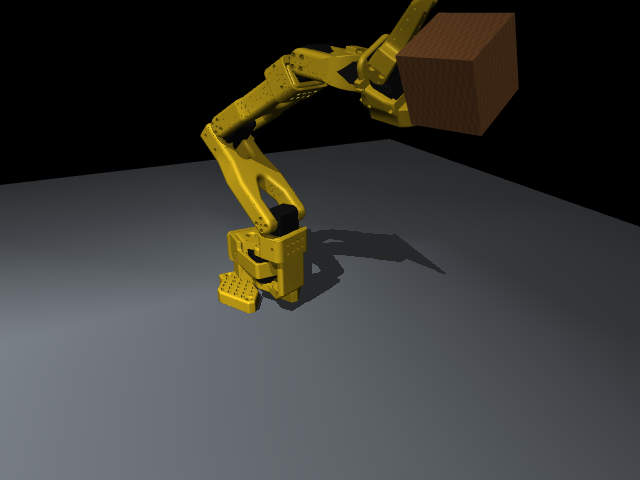
\includegraphics[width=.87\linewidth]{images/cycle.png}

\vspace{2mm}
{\smallfont\color{muted}SO-101: 5 суставов + гриппер}
\end{column}
\end{columns}
\end{frame}

\begin{frame}[t]{Инструменты и модель}
\vspace{3mm}
\begin{columns}[T,onlytextwidth]
\begin{column}{.48\textwidth}
\bodyfont
\textbf{\color{accent}MuJoCo}\\[1mm]
Физика и модель робота.

\vspace{3mm}
\textbf{\color{accent}Python, NumPy и SciPy}\\[1mm]
Обратная кинематика\\и планирование.

\vspace{3mm}
\textbf{\color{accent}RGB-D камера}\\[1mm]
Цвет, глубина и видимость.
\end{column}
\begin{column}{.47\textwidth}
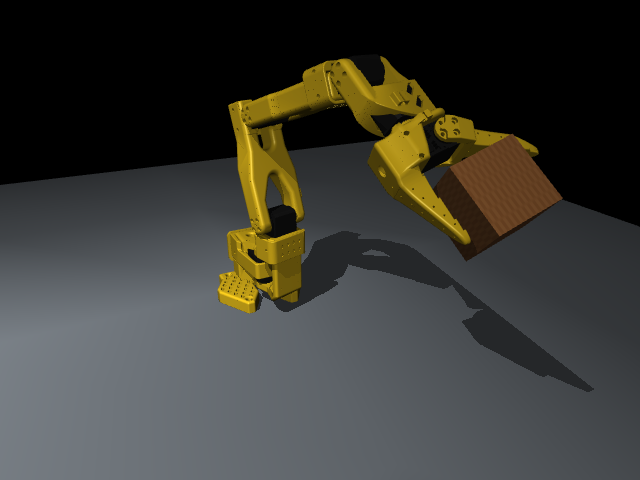
\includegraphics[width=.9\linewidth]{images/view.png}

\vspace{2mm}
{\smallfont\color{muted}Ракурс после перехвата}
\end{column}
\end{columns}
\end{frame}

\begin{frame}[t]{Архитектура}
\vspace{3mm}
{\bodyfont\color{accent}\textbf{До цикла:} библиотека захватов, ракурсов и путей}

\vspace{5mm}
\centering
\begin{tikzpicture}[
  box/.style={draw=accent!45,fill=pale,rounded corners=1mm,
    line width=.7pt,text width=3.2cm,minimum height=1.75cm,
    align=center,inner sep=1mm,font=\fontsize{13}{17}\selectfont},
  flow/.style={-{Stealth[length=2.2mm]},line width=1pt,draw=accent}
]
\node[box] (state) at (0,0) {\textbf{Состояние}\\[2mm]Позы\\и этап цикла};
\node[box] (planner) at (3.55,0) {\textbf{Планировщик}\\[2mm]Захват,\\ракурсы, пути};
\node[box] (executor) at (7.1,0) {\textbf{Исполнитель}\\[2mm]Команды\\суставам};
\node[box] (sim) at (10.65,0) {\textbf{MuJoCo}\\[2mm]Робот\\и камера};
\draw[flow] (state.east) -- (planner.west);
\draw[flow] (planner.east) -- (executor.west);
\draw[flow] (executor.east) -- (sim.west);
\draw[flow] (sim.south) -- ++(0,-1.1) -| (state.south);
\node[fill=white,inner sep=2mm,font=\fontsize{13}{17}\selectfont,text=muted]
  at (5.325,-1.92) {Обратная связь: движение и качество снимка};
\end{tikzpicture}

\vspace{2mm}
\raggedright
{\smallfont В цикле проверяем актуальную сцену перед исполнением.}
\end{frame}

\begin{frame}[t]{Управление и эффективность}
\vspace{3mm}
\begin{columns}[T,onlytextwidth]
\begin{column}{.61\textwidth}
\bodyfont
Плавная траектория\\положения и скорости.

\vspace{3mm}
PD-регуляторы суставов\\исправляют ошибку.

\vspace{3mm}
Проверка захвата\\и управляемая остановка.
\end{column}
\begin{column}{.32\textwidth}
{\fontsize{28}{30}\selectfont\bfseries\color{accent}3,4 с}\\[2mm]
{\fontsize{13}{16}\selectfont планирование\\вместо 28,2 с}

\vspace{4mm}
{\fontsize{28}{30}\selectfont\bfseries\color{accent}38 с}\\[2mm]
{\fontsize{13}{16}\selectfont движения\\полного цикла}
\end{column}
\end{columns}
\vspace{2mm}
{\fontsize{11}{14}\selectfont\color{muted}Замеры в симуляции с идеальным удержанием куба.\\Контактный захват ещё требует доводки.}
\end{frame}

\begin{frame}[t]{Алгоритм и регулятор}
\vspace{2mm}
\begin{columns}[T,onlytextwidth]
\begin{column}{.44\textwidth}
\fontsize{14}{18}\selectfont
\textbf{\color{accent}Алгоритм}

\vspace{4mm}
1. Больше покрытия\\за меньшее время.

\vspace{4mm}
2. Обратная кинематика:\\углы суставов.

\vspace{4mm}
3. Плавный путь\\и обратная связь.
\end{column}
\begin{column}{.51\textwidth}
\fontsize{14}{18}\selectfont
\textbf{\color{accent}PD-регулятор}
\setlength{\abovedisplayskip}{2mm}
\setlength{\belowdisplayskip}{2mm}
\[
\begin{aligned}
e &= q_d-q,\\
\dot e &= \dot q_d-\dot q,\\
\tau &= \operatorname{sat}(K_p e+K_d\dot e+b).
\end{aligned}
\]
{\fontsize{11}{15}\selectfont\color{muted}
\(q_d,q\): заданные и измеренные углы.\\
\(K_p,K_d\): коэффициенты регулятора.\\
\(b\): компенсация динамики модели.\\
\(\operatorname{sat}\): ограничение момента.}
\end{column}
\end{columns}
\end{frame}

\end{document}
